\documentclass[conference]{IEEEtran}
\IEEEoverridecommandlockouts
% The preceding line is only needed to identify funding in the first footnote. If that is unneeded, please comment it out.
\usepackage{cite}
\usepackage{amsmath,amssymb,amsfonts}
\usepackage{algorithmic}
\usepackage{graphicx}
\graphicspath{{./figures/}{IR}}
\usepackage{textcomp}
\usepackage{xcolor}
\usepackage{hyperref}
\def\BibTeX{{\rm B\kern-.05em{\sc i\kern-.025em b}\kern-.08em
    T\kern-.1667em\lower.7ex\hbox{E}\kern-.125emX}}
\bibliographystyle{IEEEtran}

\newcommand{\panayot}[1]{\textcolor{blue}{#1}}


\begin{document}

\title{Culinary Computation\\
{\footnotesize \textsuperscript{*}Data Analysis for Novel Recipe Generation}
\thanks{Portland State University Undergraduate Research Mentorship Program}
}

\author{\IEEEauthorblockN{1\textsuperscript{st} Nelson}
\IEEEauthorblockA{\textit{Maseeh College of Engineering and Computer Science} \\
\textit{Portland State University}\\
Portland, United States\\
ajn6@pdx.edu}
\and
\IEEEauthorblockN{2\textsuperscript{nd} Vassilevski}
\IEEEauthorblockA{\textit{Fariborz Maseeh Department of Mathematics and Statistics} \\
\textit{Portland State University}\\
Portland, United States\\
panayot@pdx.edu}
}

\maketitle

\begin{abstract}
Data utilization continues to become increasingly important as the rate of collection and
transmission rapidly expand. Much work has been done investigating algorithmic creativity for
music composition, visual artwork, and prose generation. This paper explores the potential
of algorithmic generation and modification of recipes by describing the process of data
collection, initial analysis, and processing technique.
\end{abstract}

\begin{IEEEkeywords}
graph, algebraic multigrid, data science, computational creativity
\end{IEEEkeywords}

\section{Introduction}
Food is a central component of the human condition. Its expression acknowledges no barriers
and is a defining component of all cultural experience. The US restaurant industry currently
employs over 11 million individuals \cite{BoL}.
Understanding flavor theory and developing recipes isn't difficult for a trained professional
but there is potential for improvement through utilization of data analysis. This is especially
true for large corporate chains with extensive historical data.

\section{Data Collection}
Recipes were scraped from allrecipes and New York Times Cooking (NYTC). The allrecipes database is
user created with around 60000 recipes. The NYTC database has around 18000 recipes and is
curated and maintained by journalists. Another aggregated database curated by Majumder et al.
\cite{Majumder19} was also used.

\section{Data Wrangling}
The scraped recipes are in the form of a list of strings for ingredients and procedure.
The quantity, ingredient, and adjectives were parsed from each ingredient in the ingredient
list using a conditional random field (CRF),
a discriminative probabilistic model that trains parameters using a convex loss function such
as maximum log likelihood. CRFs are a popular natural language processing
technique used for sentence parsing, names entity recognition, and segmentation \cite{Lafferty01}.
In this example, a possible phrase to be parsed could be: 3 cups carrots, chopped. This phrase is
converted into a vector of words $[w_1,w_2,w_3,w_4]$ and the desired feature output would be $[quantity, measurement, ingredient, preparation]$.
The model is trained on many phrase---feature vectors and creates feature functions for many feature---word combination.
These feature functions are weighted through training to determine the probability that any word is a feature based on its value and context.

This process isn't perfect but yields high enough quality results to create the necessary
data structures. Each unique ingredient in the database is given an ID and the recipes are
converted into lists of IDs. Alternatively, we may view the same database as a bipartite graph or equivalently as a rectangular relation  matrix "{\em recipe\_ingredient}".
Its transpose represents the relation "{\em ingredient\_recipe}". We place integer value one to indicate that two objects (recipe and ingredient) are related and zero otherwise.
Due to the zero entries, it is useful to represent these relations as sparse matrices. 

Using this new database an ingredient co-occurrence graph is constructed and represented as a weighted 
adjacency matrix. This is a symmetric matrix with a diagonal of 0s and each off-diagonal 
entry or weight  represents the number of times the two related ingredients (in the respective row and column of the matrix)  appeared in a same recipe.
Note that this adjacency matrix representing the relation "{\em ingredient\_ingredient}" can be obtained by multiplying the sparse matrices 
 "{\em ingredient\_recipe}" and "{\em recipe\_ingredient}" (we ignore the diagonal). 

To illustrate the concept, consider the following chicken recipes:

\vspace{.5cm}
\begin{tabular}{ l|l|l }
   Recipe 0    & Recipe 1        & Recipe 2  \\
   \hline
   chicken     & chicken         & chicken   \\
   lemon       & salt            & butter    \\
   salt        & pepper          & salt      \\
   pepper      & garlic          & pepper    \\
   olive oil   & honey           & garlic    \\
   oregano     & water           & paprika   \\
   parsley     & rice vinegar    &           \\
               & soy sauce       &
\end{tabular}

\vspace{.5cm}
\begin{tabular}{ l l l }
   \multicolumn{3}{c}{All unique ingredients with IDs}          \\
   \hline
   0  --- chicken  & 1  --- lemon         & 2  --- salt         \\
   3  --- pepper   & 4  --- olive oil     & 5  --- oregano      \\
   6  --- parsley  & 7  --- garlic        & 8  --- honey        \\
   9  --- water    & 10 --- rice vinegar  & 11 --- soy sauce    \\
   12 --- butter   & 13 --- paprika       &
\end{tabular}

\vspace{.5cm}
Resulting bipartite recipe\_ingredient relation:
$$
   \setcounter{MaxMatrixCols}{15}
   \begin{bmatrix}
      1 & 1 & 1 & 1 & 1 & 1 & 1 & - & - & - & - & - & - & - \\
      1 & - & 1 & 1 & - & - & - & 1 & 1 & 1 & 1 & 1 & - & - \\
      1 & - & 1 & 1 & - & - & - & 1 & - & - & - & - & 1 & 1
   \end{bmatrix}
$$

\vspace{.5cm}
Resulting co-occurrence matrix:
$$
   \begin{bmatrix}
      - & 1 & 3 & 3 & 1 & 1 & 1 & 2 & 1 & 1 & 1  & 1  & 1  & 1  \\
      1 & - & 1 & 1 & 1 & 1 & 1 & - & - & - & -  & -  & -  & -  \\
      3 & 1 & - & 3 & 1 & 1 & 1 & 2 & 1 & 1 & 1  & 1  & 1  & 1  \\
      3 & 1 & 3 & - & 1 & 1 & 1 & 2 & 1 & 1 & 1  & 1  & 1  & 1  \\
      1 & 1 & 1 & 1 & - & 1 & 1 & - & - & - & -  & -  & -  & -  \\
      1 & 1 & 1 & 1 & 1 & - & 1 & - & - & - & -  & -  & -  & -  \\
      1 & 1 & 1 & 1 & 1 & 1 & - & - & - & - & -  & -  & -  & -  \\
      2 & - & 2 & 2 & - & - & - & - & 1 & 1 & 1  & 1  & 1  & 1  \\
      1 & - & 1 & 1 & - & - & - & 1 & - & 1 & 1  & 1  & -  & -  \\
      1 & - & 1 & 1 & - & - & - & 1 & 1 & - & 1  & 1  & -  & -  \\
      1 & - & 1 & 1 & - & - & - & 1 & 1 & 1 & -  & 1  & -  & -  \\
      1 & - & 1 & 1 & - & - & - & 1 & 1 & 1 & 1  & -  & -  & -  \\
      1 & - & 1 & 1 & - & - & - & 1 & - & - & -  & -  & -  & 1  \\
      1 & - & 1 & 1 & - & - & - & 1 & - & - & -  & -  & 1  & -
   \end{bmatrix}
$$

We note that the above example creates an ingredient co-occurrence relation based on one class of recipes (namely the {\em chicken} ones).
It is clear that one may involve recipes that come from different classes (e.g., from desert menu, salads, soups, etc.)

\section{Initial Exploration}
The first goal of the study is to confirm and explore the expectation that there are meaningful
relationships between the ingredients that we choose to combine into recipes. Previous research
by Ahn et al.  \cite{Ahn11} has focused on the relationship of ingredients and the flavor compounds
they contain on a geographical basis and concluded that Western cuisine pairs ingredients with
similar compounds and Southern Europe/Eastern Asia often avoid these pairings. Ahn et al. also
identified that there are core authentic pairs and triplets of ingredients that can define a
region's cuisine and these core groupings are largely responsible for the difference discovered
in the primary conclusion.

We identify relationships between ingredients through multilevel community detection of
the ingredient co-occurrence graph and visualize these communities by embedding them into a three
dimensional space. The coarsening algorithm used is described in \cite{Quiring19modularity} which utilizes
optimizing of modularity to hierarchically aggregate vertices. Modularity of a clustered graph
is a scalar that represents the quality of the clustering. High modularity means there are many
edges between vertices within the aggregates and few edges between the aggregates themselves.
When any two vertices are joined to make a new aggregate, all the edges are brought along and
if both had edges to a mutual vertex the new weight to the mutual vertex is the sum of those
edges.

Following is an overview of the algorithm to select vertices to merge to maximize
the modularity as described in \cite{Quiring19modularity}.
\begin{align}
   \intertext{The ingredient co-occurrence matrix is a symmetric $n \times n$ matrix $A = (a_{ij})$.
   First, the rowsums of A are calculated. These rowsums make $r \in \mathbb{R}^n$.}
   r_i &= \sum_j a_{ij}
   \intertext{Let the total rowsum be}
   T &= \sum_i r_i
   \intertext{And the normalized rosums}
   \alpha_i &= \frac{r_i}{T}
   \intertext{The modularity matrix, $B = (b_{ij})$, is defined}
   B &= A - \frac{1}{T}rr^T
   \intertext{Now consider a non-overlapping partition of the vertex set $\{\mathcal{A}\}$.
   The new normalized rowsum and aggregate edges of each aggregate, $\mathcal{A}$}
   \alpha_\mathcal{A} &= \frac{1}{T}\sum_{i \in \mathcal{A}} r_i\\
   a_{\mathcal{A}\mathcal{B}} &= \sum_{i \in \mathcal{A}} \sum_{j \in \mathcal{B}} a_{ij}
   \intertext{The modularity of the partition, $\mathcal{Q}$, is}
   \mathcal{Q} &= \frac{1}{T}\sum_\mathcal{A}\sum_{i \in \mathcal{A}}\sum_{j \in \mathcal{A}}b_{ij}
   \intertext{The goal of the algorithm is to select the next partitioning to maximize the
   change of modularity. To do so we create the change of modularity matrix, $\Delta\mathcal{Q}$.
   Both $B$ and $\Delta \mathcal{Q}$ have the desirable property of zero rowsums.
   Consider merging aggregates $\mathcal{A}$ and $\mathcal{B}$ from $\{A\}$. The resulting
   change in modularity, $\Delta \mathcal{Q}_{\mathcal{A} \mathcal{B}}$}
   \Delta \mathcal{Q}_{\mathcal{A} \mathcal{B}} &= 2\left(\frac{a_{\mathcal{A}\mathcal{B}}}{T} - 
   \alpha_\mathcal{A} \alpha_\mathcal{B}\right)
   \intertext{Using $\Delta\mathcal{Q}$ we can find which aggregate pairs should be merged by
   looking for the maximum value of each row. Construct the vector, $p = (p_i)$, which contains
   the maximum positive value from $\Delta\mathcal{Q}_{ij}$ for that row. If no positive values
   exist then $p_i = -1$.}
   p_i &= argmax\{\Delta\mathcal{Q}_{ij} | \Delta\mathcal{Q}_{ij} > 0\}
   \intertext{This p vector can be used to construct the piecewise constant interpolation matrix,
   $P = (p_{ij})$. All pairs where $p_i = j$ and $p_j = i$ will be merged to create $A_c$. $P$
   is a sparse $n \times n_c$ matrix where each column is a aggregate in the coarsened graph.
   These columns will have all $0$'s with $1$ at each $i$ in the aggregate. This gives us}
   A_c &= P^TAP\\
   \Delta \mathcal{Q}_c &= \frac{2}{T}A_c - \frac{2}{T^2}r_cr^{T}_{c}
\end{align}

The efficiency of this algorithm comes from exploiting the sparse triple matrix
product $P^TAP$ and matrix vector products to construct $r_c = P^Tr$, which can both be calculated
in parallel.

Steps 9 through 11 are
repeated to give a hierarchy of partitions. The algorithm completes when there is no
positive values in $\Delta \mathcal{Q}$. Note that because $\Delta \mathcal{Q}$ has 0 rowsums, 
it is a weighted graph Laplacian and the modularity, $\mathcal{Q}$, is the sum of the diagonal.
The algorithm can be terminated early if the coarsening factor isn't below a desired value.
If $A$ is $n \times n$ and $A_c$ is $m \times m$ the coarsening factor is $\frac{m}{n}$.
Other heuristics can be applied to speed the coarsening such as increasing the number of passes
when constructing the $p$ joining vector, starting with leaf aggregation at each level, and
applying random weights to $\Delta \mathcal{Q}$ at each level.

To visualize the structure of this network these partitions were embedded into a three 
dimensional space using a multilevel approach as described in \cite{Quiring19embed} using
a multilevel adaptation to the ForceAtlas2 algorithm from Gephi. \textbf{need citation?}

When processing an entire
database with these algorithms, little structure was identified and most of the vertices
aggregated to hubs of commonly found ingredients. This is expected, as certain ingredients such as sugar, butter, and
flour are extremely common. When a database was filtered by tags such as cuisine or recipe class clear structure
was identified. Some clusterings such as filtering by pasta, salad, and cocktail result in
tightly grouped clusters that contain intuitive groups of ingredients demonstrating there is
{\panayot{describe some ingredients that are colored the same in  the figures}} \ref{fig:P1compileP0-1}-\ref{fig:P2compileP0-1}. 
structure in the network of ingredient relationships.

  \begin{figure}[h!]
	\centering
	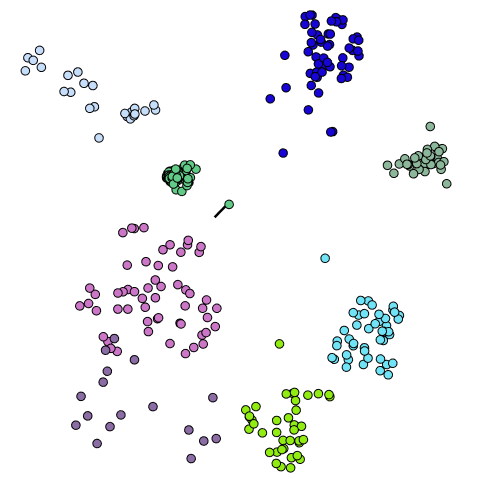
\includegraphics[width=0.8\linewidth]{pastas.png}
	\caption[Embedding of ingredients in pasta recipes]{Embedding of ingredients in pasta recipes}
	\label{fig:P2compileP0-1}
  \end{figure}

  \begin{figure}[h!]
	\centering
	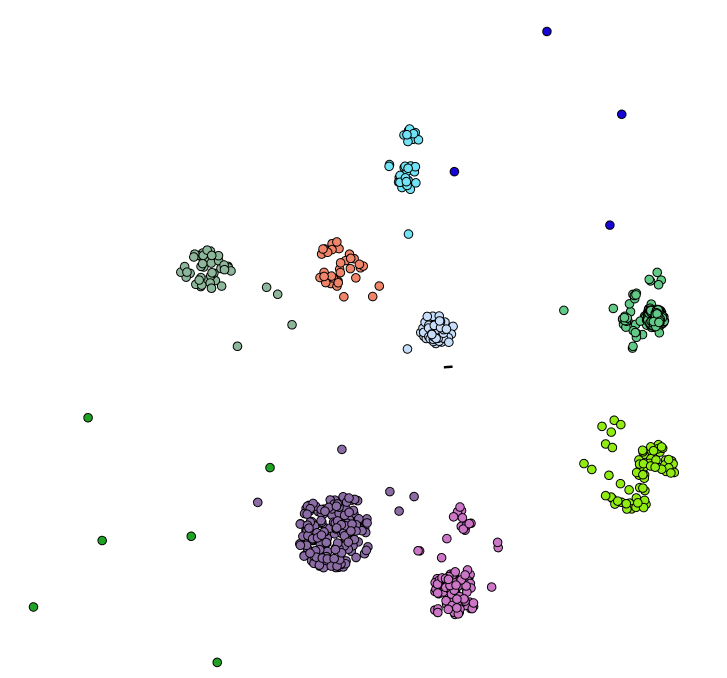
\includegraphics[width=0.8\linewidth]{salads.png}
	\caption[Embedding of ingredients in salad recipes]{Embedding of ingredients in salad recipes}
	\label{fig:P2compileP0-1}
  \end{figure}


\section{From ingredient co-occurrence relations back to recipes}
Our first study is after we generate ingredient co-occurrence relations based on a class of recipes, to recover these recipes (and perhaps some new ones).
For this we use some community detection algorithms, namely \cite{blondel08}. In our setting, community should translate to recipe. With the 
co-occurrence graphs though, applying  community detection  algorithms will result to communities that partition the graph into non-overlapping vertex
sets which means they have no chance to represent all of the original recipes  since with this approach an ingredient can belong to exactly a  single community.
Note that we create the co-occurrence graphs using recipes that generally have  some common ingredients. 

To allow a vertex (i.e. ingredient) to participate in several communities, we embed the co-occurrence graph into a larger one.
First, each vertex $i$ is cloned into $m_i$ new vertices, where $m_i$ is the number of recipes it  participates  originally. 
Now, we have that the original vertex is replaced by a node of $m_i+1$ vertices which represent the same vertex $i$.
We connect them in a star-shaped manner (we could use clique as well); the original vertex is connected to the new $m_i$ vertices
by adding new $m_i$ edges to the original co-occurrence graph.  Each new vertex $i{'}$ from the node $i$ is labeled with a label
representing the original recipe it corresponds to.  That is, the  recipes used to generate the original ingredient co-occurrence graph have their label. 

Now, consider any original pair of connected vertices, $i$ and $j$, i.e., consider an original edge $(i,j)$. 
We have $m_i$ and $m_j$ new vertices connected to $i$ and $j$ respectively. 
If a new vertex $i{'}$ from the node $i$ and a new vertex $j{'}$ from the node $j$, came from a same recipe, i.e., have the same label,  we create an edge between them denoted $(i{'},j{'})$ .
This allows to create as many new edges between node $i$ and $j$ as many common recipes they participate to. 

Now, we have created an embedding graph that takes into account the recipes (with their labels) that were used to create the original co-occurrence graph.   
Our goal is to find communities (old and possibly new recipes)  in this large embedding graph. Since we have multiple copies of the ingredients incorporated into
the embedding graph, the communities that we find, will have overlap which is essential to recover the original  recipes.  

\subsection{Results}

When optimizing modularity with the Louvain method as described in \cite{blondel08}, the original recipes are identified and become communities in the first iteration of the
algorithm (level one of the hierarchy). The second iteration merges recipes that share multiple ingredients. This is expected because the vertices that make up the ingredients
of any recipe make a clique and the vertex class for any ingredient forms a star. 

\section{Using graph embedding for recipe generation with some desired ingredients}
In this section, we consider the following task.
We are interested to create a recipe that contains some ingredients that we like. 
That is, we are given some initial set of ingredients that we refer to as target ingredients. Using our database, we identify recipes that contain some (at least one) of  the target ingredients.
We label the recipes we identified. Then, use the ingredients of the identified recipes to form the corresponding relation "{\em recipe\_ingredients}"
and from it the corresponding co-occurrence relation "{\em ingredient\_ingredient}". Note that our initial set of ingredients is a subset of the vertices of the last graph.
Since we want to increase the chance of these target ingredients to end up in a same community (i.e., recipe) we fully  connect them to form a clique and add these new edges
to the constructed co-occurrence graph. For this graph and the identified (labeled) recipes we build the embedding graph as described in the previous section and find its communities.
We identify the communities (one or more) that contain most of the  initial ingredients. Those would be our proposed new recipes (one or more). 

\subsection{Results}

When connecting the target ingredients as a clique they were all grouped into one community
in the first iteration of Louvain's and the remaining ingredients in each recipe (that are also
connected with a clique) would be grouped as well. The result is on further iterations of the
algorithm was simply combining entire recipes that shared the most ingredients. The idea of
expanding the relation was to "loosen" the structure so this result isn't desirable and could
be obtained through calculating the similarity of the recipe vectors. To even out the structure
of the graph all cliques were converted into stars. Consider the expanded graph from section five
before the edges between vertices from the same recipe were added. Instead, a new node is added
for each recipe and the expanded vertices are connected to their respective recipe node to create
recipe stars. For connecting the target ingredients in section six, a similar procedure is done.
Instead of connecting all the target ingredients in a clique, a new node for the target hub
is created and the target ingredient hubs are connected to it in star like manner. The resulting
graph has no cliques with more than 2 nodes. This new expanded graph has a very homogeneous
structure and in the first pass of Louvain's each node has an equal affinity for grouping
with it's neighbors. Because Louvain's visits each node in a random order each iteration of the
graph, there can be significant variation in the resulting partitions between various runs of
the algorithm. By the second iteration of Louvain's there is usually one (large) community with
all the target ingredients and many smaller communities with at least one of the targets. 

\textbf{An example:}

When filtering by the tag "Asian" and target ingredients of Chicken, Soy Sauce, Brown Sugar
(Chicken Teriyaki like dish) the top 25 ingredients in the community with all targets are:
\begin{itemize}
\item 70 - soy sauce
\item 52 - scallions
\item 51 - ginger
\item 48 - sesame oil
\item 38 - garlic
\item 31 - chicken
\item 21 - rice vinegar
\item 17 - salt
\item 14 - peanut oil
\item 13 - dry sherry
\item 13 - sugar
\item 13 - sesame seeds
\item 12 - brown sugar
\item 12 - black pepper
\item 10 - chicken stock
\item 8 - cornstarch
\item 8 - cilantro
\item 7 - oil
\item 6 - water
\item 6 - vegetable oil
\item 6 - red pepper flakes
\item 4 - tabasco sauce
\item 4 - oysters
\item 4 - lemon
\item 4 - coriander
\end{itemize}

When looking at the first 8 ingredients to see if any recipe has all of the ingredients none
is found. This means that the top 8 ingredients of this community form an original recipe.
This recipe seems pretty sensible. The seasoning selection is quite simple but hits the
fundamentals of what I would expect. Coriander, lemon, tabasco, cilantro, black pepper, sesame
seeds, sherry, and garlic would definitely work. Corn starch is included to thicken the sauce.
The redundancies of cooking oils could be eliminated. Oysters is an addition I wouldn't have
thought of but probably adds some umami with a decent dose of glutamates.

\subsection{Thoughts}
I was having the problem that I described where the cliques in the expanded relation were
being aggregated quickly and ignoring the loosening effect of expanding the graph. To mitigate
this I "balanced" the graph by eliminating all cliques and replaced everything with stars.

This seems to work with the limited investigation I have done but looking at the other
communities that do not contain the target ingredients there are still many communities mostly
contain nodes from single recipes.

I am thinking that I should investigate what happens if instead of moving everything to stars,
move everything to cliques. This would mean that it would still be "balanced" but there would
be more edges to consider and might have a better loosening effect. So basically:

Expand the ingredient---ingredient relation, connect all nodes from each ingredient node in a
clique, connect all nodes from each recipe in a clique, and connect all nodes from the target
ingredients in a clique. Do community detection on this extremely highly connected graph.

\section{What I am currently working on next:}
\begin{itemize}
   \item Overhauling the schema for my database so it is easier to work with. When I originally
      scraped all the recipe data I didn't have any experience using a relational database 
      management system or object-relational mapping tools. The schema I designed is bad and
      the serialization techniques I used are embarrassing. As the complexity of my analysis
      application grows it is becoming very difficult to work with the data.
   \item Creating better and more automated visualization tools. To create graphs and visualize
      my data I have been running my application and generating html files with plotly. These
      visuals are pretty primitive and I would like to make a more interactive web based app
      that lets me explore my data more efficiently.
   \item Trying the different expanded relation as described in the Thoughts section above.
   \item Trying community detection using the parallel modularity functional instead of Louvain's
      for generating recipes.
\end{itemize}

\bibliography{IEEEabrv,/home/austen/Documents/school/research/paper/references.bib}

\end{document}
